% Při kompilaci dokumentu LuaLaTeXem dojde k chybě, protože
% nedefinuje \pdfpagewidth a \pdfpageheight. 
% Balíček luatex85 to napravuje.
\RequirePackage{luatex85}
\PassOptionsToPackage{shorthands=off}{babel}
\makeatletter
\disable@package@load{fontenc}
\makeatother
\let\oldlooseness=\looseness
\documentclass{csbulletin}
\setcounter{secnumdepth}{3}
\usepackage{titlesec}
\titlelabel{\thetitle\enspace}
\usepackage{luavlna,float}
\usepackage[strict]{lua-widow-control}

\usepackage{minted}
\usemintedstyle{bw}
% \setminted{firstnumber=last, linenos}
\newenvironment{mintedblock}{%
  \let\textit\textsl
  \par\vspace{\topsep}\vspace{\partopsep}%
  \begingroup
  \fvset{listparameters=\setlength{\topsep}{0pt}\setlength{\partopsep}{0pt}}%
}{%
  \endgroup
  \par\vspace{\topsep}\vspace{\partopsep}%
}

\usepackage{csquotes}
\usepackage[
  backend=biber,
  style=iso-numeric,
  citestyle=numeric-comp,
  sortlocale=cs,
  autolang=other,
  bibencoding=UTF8,
  mincitenames=2,
  maxcitenames=2,
]{biblatex}
\addbibresource{main.bib}
\renewcommand\multicitedelim{\addsemicolon\space}

\usepackage{sideways-figure, graphicx, afterpage, subcaption, tikz}
\graphicspath{{./images/}}
\usetikzlibrary{arrows.meta}
\usetikzlibrary{decorations.pathmorphing}
\usetikzlibrary{decorations.pathreplacing}

\usepackage[
  implicit=false,
  hidelinks,
]{hyperref}
\newcommand\vref[1]{\ref{#1} na straně~\pageref{#1}}

\newcommand\pkg{\textsf}
\ExplSyntaxOn
\newcommand
  \acro
  [ 1 ]
  {
    \tl_set:Nn
      \l_tmpa_tl
      { #1 }
    \regex_replace_all:nnN
      { [^\d]+ }
      { \c{textsc} \cB\{ \c{MakeLowercase} \cB\{ \0 \cE\} \cE\} }
      \l_tmpa_tl
    \regex_replace_all:nnN
      { \d+ }
      { \c{oldstylenums} \cB\{ \0 \cE\} }
      \l_tmpa_tl
    \tl_use:N
      \l_tmpa_tl
  }
\ExplSyntaxOff

\begin{document}

\title{Příprava videozáznamu české premiéry multimediálního díla ,,Fantasia Apocalyptica``}
\EnglishTitle{Recording the Czech premiere of the ``Fantasia Apocalyptica'' multimedia work}
\author{Vít Starý Novotný}
\podpis{Vít Starý Novotný, witiko@mail.muni.cz}
\maketitle[1.5ex]

\selectlanguage{czech}
\singlechars{czech}{AaIiVvOoUuSsZzKk}

\vspace{-15pt}
\begin{abstract}
Dne 11. října 2019 se při příležitosti oslav 25. výročí založení Fakulty informatiky Masarykovy univerzity uskutečnila česká premiéra multimediálního díla ,,Fantasia Apocalyptica`` za osobní účasti autora, Donalda Knutha. Z představení byl pořízen \href{https://youtu.be/wk7dEKMPP68}{záznam}, který je dostupný na \href{https://www.youtube.com/@fi_muni}{kanálu YouTube Fakulty informatiky}.
\oldlooseness=-1

V tomto článku popisuji přípravu záznamu od akvizice a zpracování surových audiovizuálních dat přes přípravu replik panelů doprovázejících představení po spojení jednotlivých částí do výsledného záznamu. S výjimkou střihu úvodního slova a závěru, navýšení rozlišení videa a zúžení dynamického rozsahu zvuku proběhlo zpracování pomocí svobodných nástrojů jako \TeX, Audacity, Aegisub, FFmpeg, \acro{MLT}, \acro{PDF}tk a ImageMagick. V článku ukazuji užití těchto nástrojů.
\end{abstract}
\klicovaslova: audiovizuální záznam, zpracování videa, titulky, zpracování zvuku, \TeX, Audacity, Aegisub, \acro{ASS}, FFmpeg, ImageMagick, \acro{MLT}, \acro{PDF}tk, waifu2x

\bigskip

Dne 11. října 2019 se v jezuitském kostele Nanebevzetí Panny Marie uskutečnila česká premiéra multimediálního díla ,,Fantasia Apocalyptica``~\cite{knuth2023fantasia} za osobní účasti autora, Donalda Knutha. Z představení byl pořízen \href{https://youtu.be/wk7dEKMPP68}{záznam}, který je veřejně dostupný na \href{https://www.youtube.com/@fi_muni}{kanálu YouTube Fakulty informatiky~(\acro{FI~MU})}~\cite{fimu2020czech}. Předchozí články ve Zpravodaji \CSTUG u popisují průběh představení~\cite{luptak2019fantasia} a přednášek Donalda Knutha při příležitosti návštěvy Brna~\cite{szaniszlo2020dva}. V tomto článku popisuji přípravu záznamu představení.

Nejprve v sekci~\ref{sec:akvizice} popisuji akvizici a zpracování surových audiovizuálních dat. Následně v sekci~\vref{sec:uvodni-slovo-a-zaver} popisuji přípravu videozáznamu úvodního slova a závěru představení. Dále v sekci~\vref{sec:panely} popisuji přípravu panelů doprovázejících představení. Nakonec v sekci~\vref{sec:spojeni} popisuji spojení jednotlivých částí do výsledného záznamu. V sekci \vref{sec:zaver} popisuji promítání hotového videozáznamu na \acro{FI~MU} 18. prosince 2019.

\vspace{-10pt}
\section{Akvizice a zpracování videa a zvuku}
\label{sec:akvizice}
\vspace{-5pt}
Video a zvuk představení zaznamenali a předzpracovali Pavel Šiler, Petr „Tudy“ Holubář a studenti laboratoře \acro{LEMMA}~\cite{LEMMA}. Poté jsem u videa sjednotil formát dat a do zvuku jsem přimíchal zvuky okolí a úvodní slovo Jiřího Zlatušky.

\vspace{-10pt}
\subsection{Záznam videa}
Videozáznam představení pořídil Pavel Šiler na kameru Sony~\acro{PXW-X70}. Video zahrnuje přednášky Donalda Knutha na \acro{FI~MU}~\autocites{2019-10-08-video-Knuth-QA1-Sony-Siler}{2019-10-09-video-Knuth-QA2-Sony-Siler}[adresář~\texttt{staticka/}]{2019-10-11-video-Fantasia-apocalyptica-Sony-Siler}, záběry kostela a varhan a úvodní slovo Jiřího Zlatušky.

\vspace{-10pt}
\subsection{Zpracování videa}
Ačkoliv jsem video obdržel v rozlišení $1920\times1080$\,px a s frekvencí 25 snímků za sekundu, od výsledného videozáznamu se očekávalo alespoň dvojnásobné rozlišení \acro{4K} a frekvence 50 snímků za sekundu.
Záznamy přednášek jsem obdržel v prokládaném (tzv. „interlaced“) formátu, zatímco záběry kostela, varhan a úvodní slovo byly v neprokládaném (tzv. „progressive“) formátu. Přednášky a úvodní slovo byly dále natáčeny ze stativu, na rozdíl od záběrů kostela a varhan, které byly pořízeny z ruky. Cílem zpracování videa bylo nejen navýšení rozlišení a snímkové frekvence, ale také sjednocení formátu videa a stabilizace záběrů z ruky.

Video jsem zpracoval svobodným nástrojem FFmpeg~\cite{ffmpeg} a otevřeným nástrojem waifu2x~\cite{waifu2x}, vizte obrázky~\ref{fig:ffmpeg-waifu2x}--\ref{fig:minterpolate-yadif}. Nejprve jsem stabilizoval záběry z ruky filtry \texttt{vidstabdetect}~\cite{vidstabdetect} a~\texttt{vidstab\discretionary{\textrm{-}}{}{}transform}~\cite{vidstabtransform} nástroje FFmpeg. Potom jsem navýšil rozlišení a snímkovou frekvenci následujícím způsobem:\footnote{Navýšené rozlišení a především snímková frekvence jsou jen iluze. Proto upravené video tvoří jen ca 7 minut ze 104minutového videozáznamu. Zbylých 97 minut tvoří animované panely, které mají nativní rozlišení \acro{4K} a snímkovou frekvenci 50 snímků za sekundu.}
\begin{itemize}
\item U neprokládaných videí jsem nejprve navýšil rozlišení nástrojem waifu2x. Následně jsem navýšil snímkovou frekvenci filtrem \texttt{minterpolate}~\cite{minterpolate} nástroje FFmpeg, který chybějící snímky interpoluje podle okolních snímků.
\item U prokládaných videí jsem nejprve navýšil snímkovou frekvenci filtrem \texttt{yadif}~\cite{yadif}, který chybějící půlsnímky interpoluje podle okolních půlsnímků a řádků. Nakonec jsem navýšil rozlišení nástrojem waifu2x.
\end{itemize}

\begin{figure}[t!]
\vspace{-10pt}
\input images/ffmpeg-waifu2x-activity-diagram
\caption{Diagram aktivit zpracování videa pomocí nástrojů FFmpeg a waifu2x.}
\label{fig:ffmpeg-waifu2x}
\end{figure}

\subsection{Záznam zvuku}
Zvuk představení byl zaznamenán šesti mikrofony:
\begin{itemize}
    \item \textls[-2]{Dva mikrofony Zoom~\acro{H1}~\cite{2019-10-11-audio-Fantasia-apocalyptica-ZoomH1-TS} byly umístěny na řečnickém pultu a nad panely.}
    \item Dva mikrofony Oktava~\acro{MK012}~\cite[soubor~\texttt{ORTF-MK012\_nearReversed.flac}]{2019-10-11-audio-Fantasia-apocalyptica-Mix-Tudio} \textls[-15]{byly zapojeny do rekordéru Zoom~\acro{H4}, umístěny na kůru a namířeny do kostela.}
    \item Mikrofon Roland~\acro{R26}~\cite{2019-10-11-audio-Fantasia-apocalyptica-RolandR26zLemma-organ} a mikrofon kamery Sony~\acro{PXW-X70}~\cite{2019-10-11-audio-Fantasia-apocalyptica-Sony-Siler} byly umístěny na kůru a namířeny na varhany.
\end{itemize}

Zvuk předzpracoval Petr „Tudy“ Holubář~\cite{2019-10-11-audio-Fantasia-apocalyptica-Mix-Tudio}. Hlavním vstupem jeho mixu byl prostorový záznam z mikrofonů Oktava~\acro{MK012}. Do prostorového záznamu Petr pro konkrétnost lehce přimíchal přímý záznam varhan z mikrofonu Roland~\acro{R26}, který frekvenčně ošetřil tak, aby se neprojevily nežádoucí fázové posuny ve spodním pásmu. Pro zúžení dynamického rozsahu použil Petr digitální \acro{VST} modul \acro{SSL}~G-Master Buss Compressor~\cite{ssl-g-master-buss-compressor} od firmy Waves Audio.

\subsection{Zpracování zvuku}
Zvuk jsem zpracoval svobodným programem Audacity~\cite{2019-11-19-audio-Fantasia-apocalyptica-Mix-Novotny,2019-12-09-audio-Fantasia-apocalyptica-Mix-Novotny}, vizte Obrázek~\ref{fig:audacity}. Výsledný mix zahrnuje svobodný zvuk zvonu kostnické katedrály~\cite{edsward2016church}, předzpracovaný zvuk představení od Petra Holubáře a úvodní slovo Jiřího Zlatušky podkreslené zvuky okolí z mikrofonů Oktava~\acro{MK012}.

\section{Příprava videozáznamu úvodního slova a závěru}
\label{sec:uvodni-slovo-a-zaver}
Videozáznam úvodního slova a závěru jsem připravil se Šimonem Mačejovským.

\subsection{Střih úvodního slova a závěru}
Videozáznamy úvodního slova a závěru~\cite{2019-12-24-video-strih-4k-Macejovsky} připravil Šimon Mačejovský nástrojem Sony Vegas 15. Videozáznam obsahuje záběry z přednášek Donalda Knutha na \acro{FI~MU}, záběry kostela a varhan, úvodní slovo Jiřího Zlatušky a fotografie od Martiny Morávkové~\cite{2019-10-08-foto-dek1-Morávková}.

\subsection{Titulky úvodního slova}
\begin{filecontents}[overwrite,nosearch,noheader]{example-ass.sh}
$ ffmpeg -i vstupní-video.mp4 -vf ass=vstupní-titulky.ass video-s-titulky.mp4
\end{filecontents}
Úvodní slovo Jiřího Zlatušky jsem opatřil titulky ve formátu \acro{ASS}\footnote{Pro vypálení titulků do obrazu videa slouží filtr \texttt{ass} nástroje FFmpeg:
\begin{mintedblock}
\inputminted{text}{example-ass.sh}
\end{mintedblock}
\noindent
Filtr \texttt{ass}~\cite{ass} implementuje softwarová knihovna \texttt{libass}~\cite{libass}, která ve výchozím nastavení nepoužívá kerningovou tabulku použitého písma~\cite{enable-kerning-by-default}. Pro použití kerningové tabulky je třeba do sekce \texttt{[Script Info]} souboru \texttt{vstupní-titulky.ass} přidat řádek \texttt{Kerning: yes}.}~\cite{2019-12-12-titulky-Novotny}, které jsem připravil ve svobodném nástroji Aegisub~\cite{aegisub}, vizte Obrázek~\ref{fig:aegisub}.

\input images/ffmpeg-waifu2x

\begin{sideways-figure}{fig:audacity}
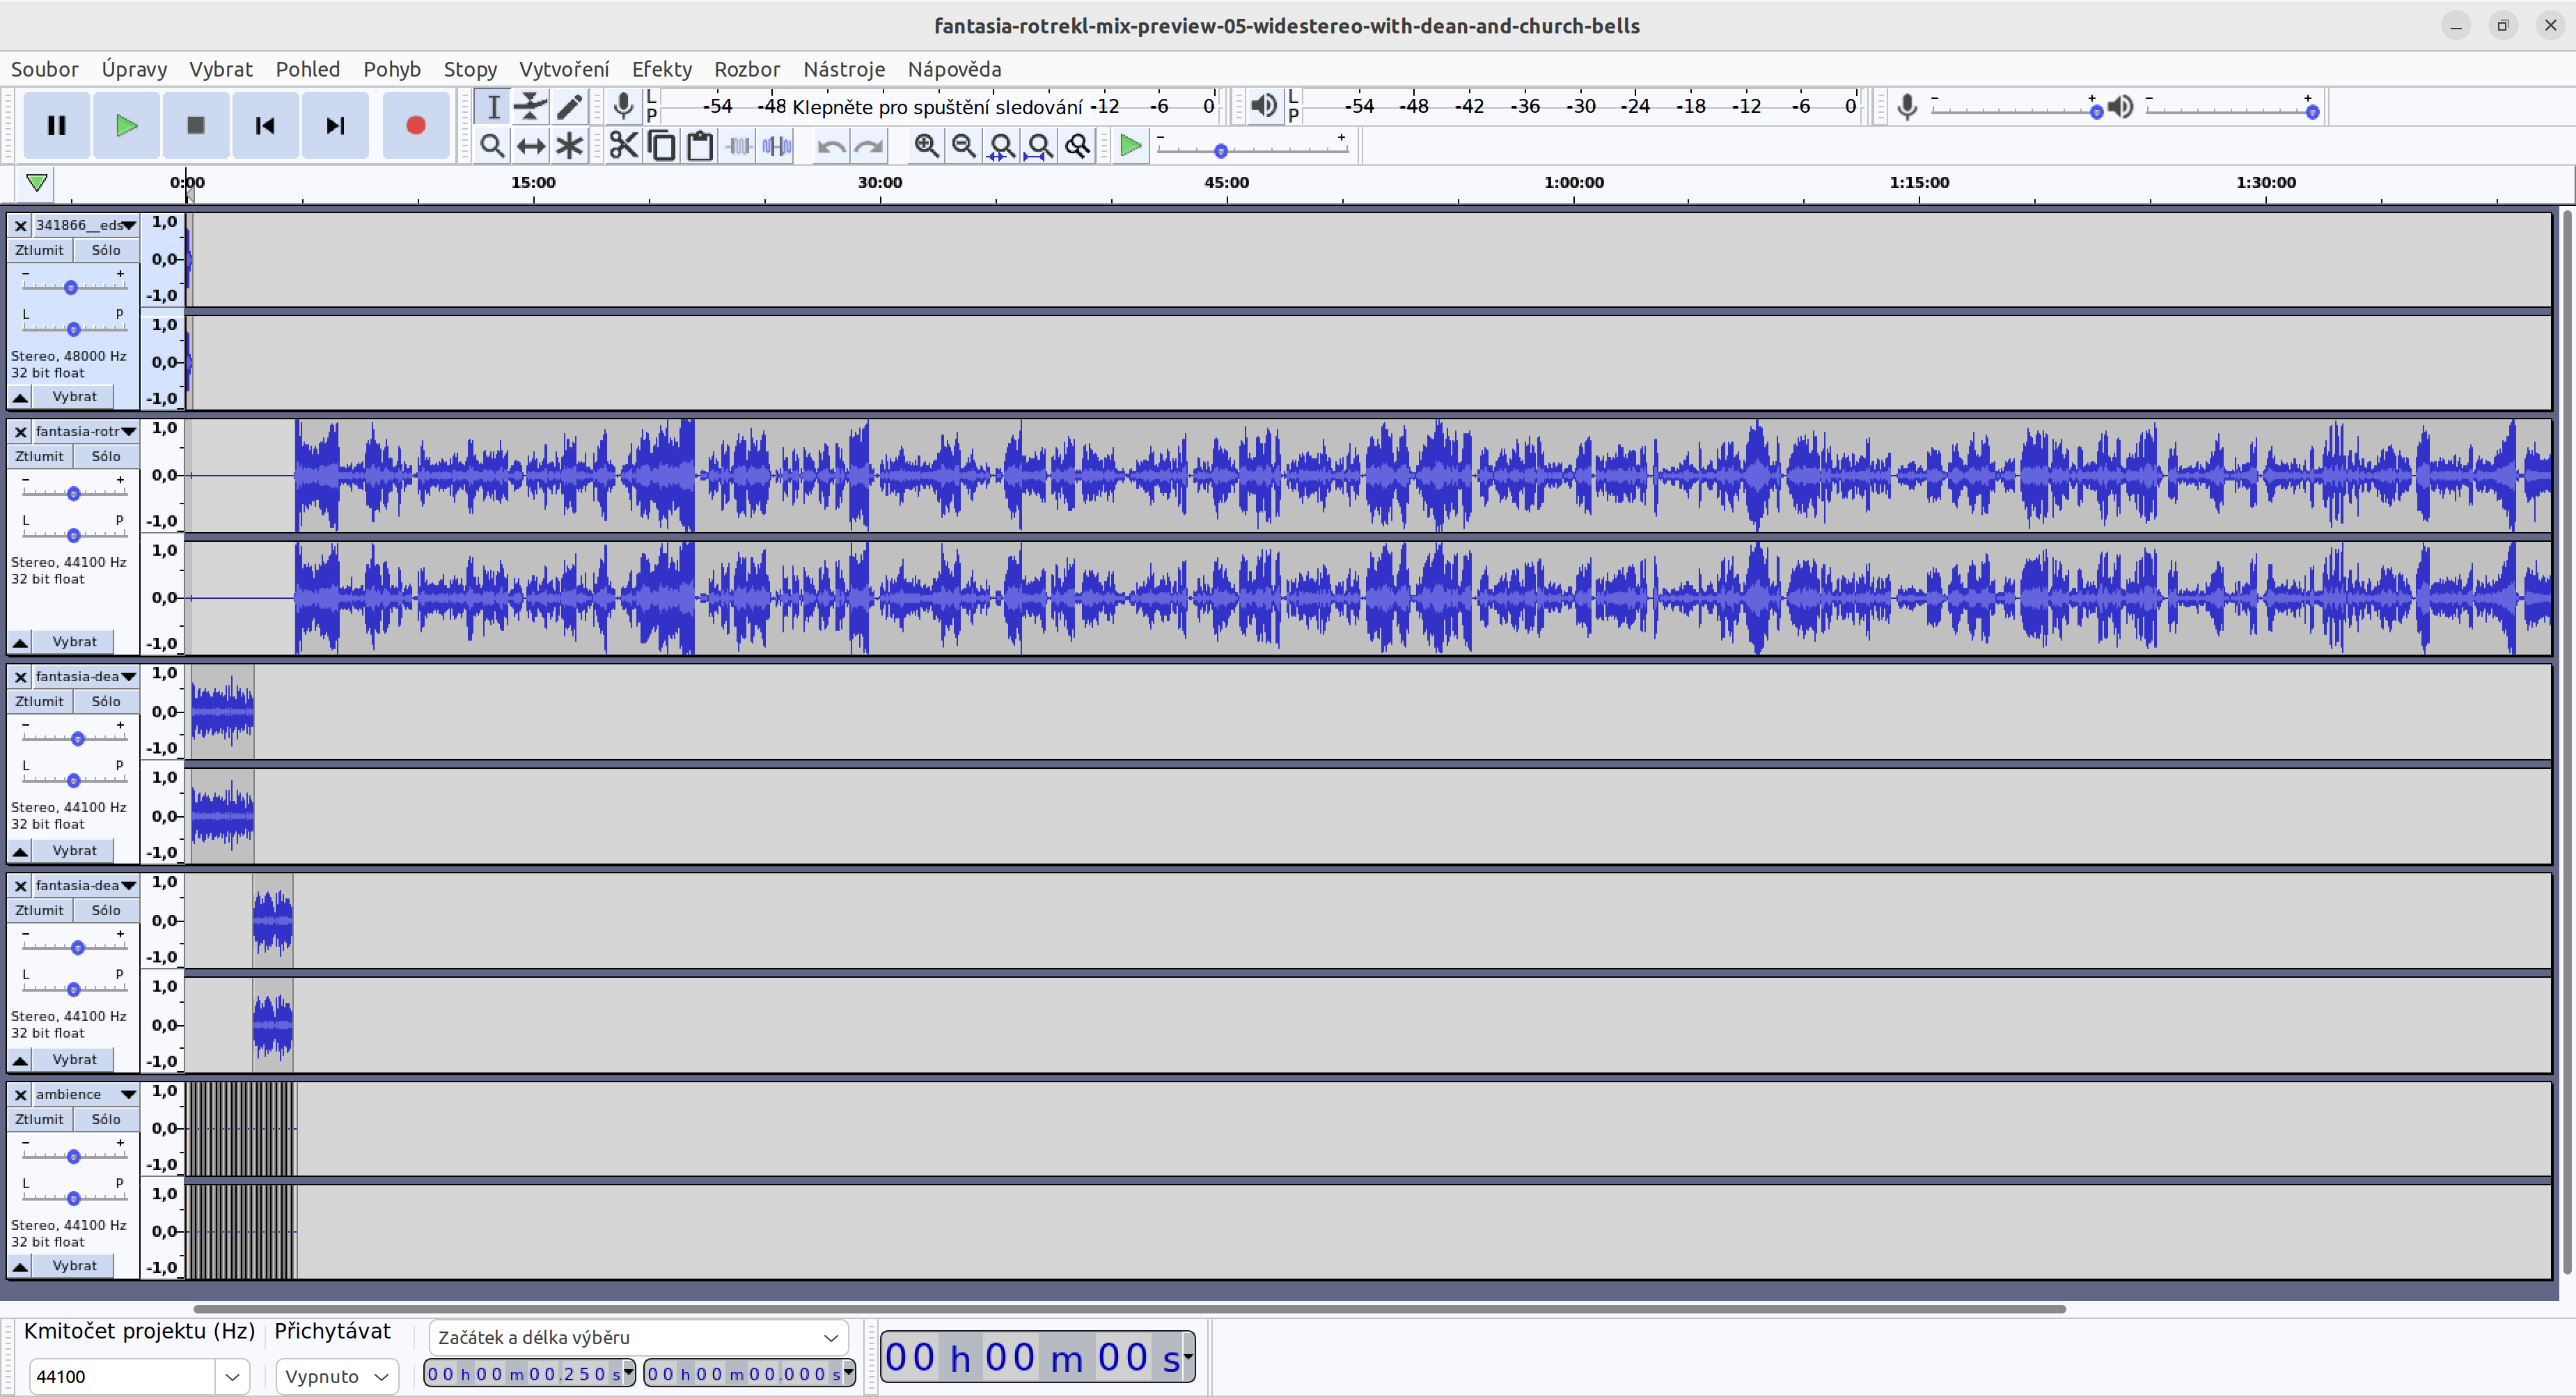
\includegraphics[width=\linewidth]{audacity}
\caption{Zpracování zvuku ve svobodném programu Audacity. Výsledný mix zahrnuje zvuk zvonu (nahoře), předzpracovaný zvuk představení od Petra „Tudy“ Holubáře (druhý odshora) a úvodní slovo Jiřího Zlatušky (uprostřed) podkreslené zvuky okolí (dole).}
\end{sideways-figure}

\begin{sideways-figure}{fig:aegisub}
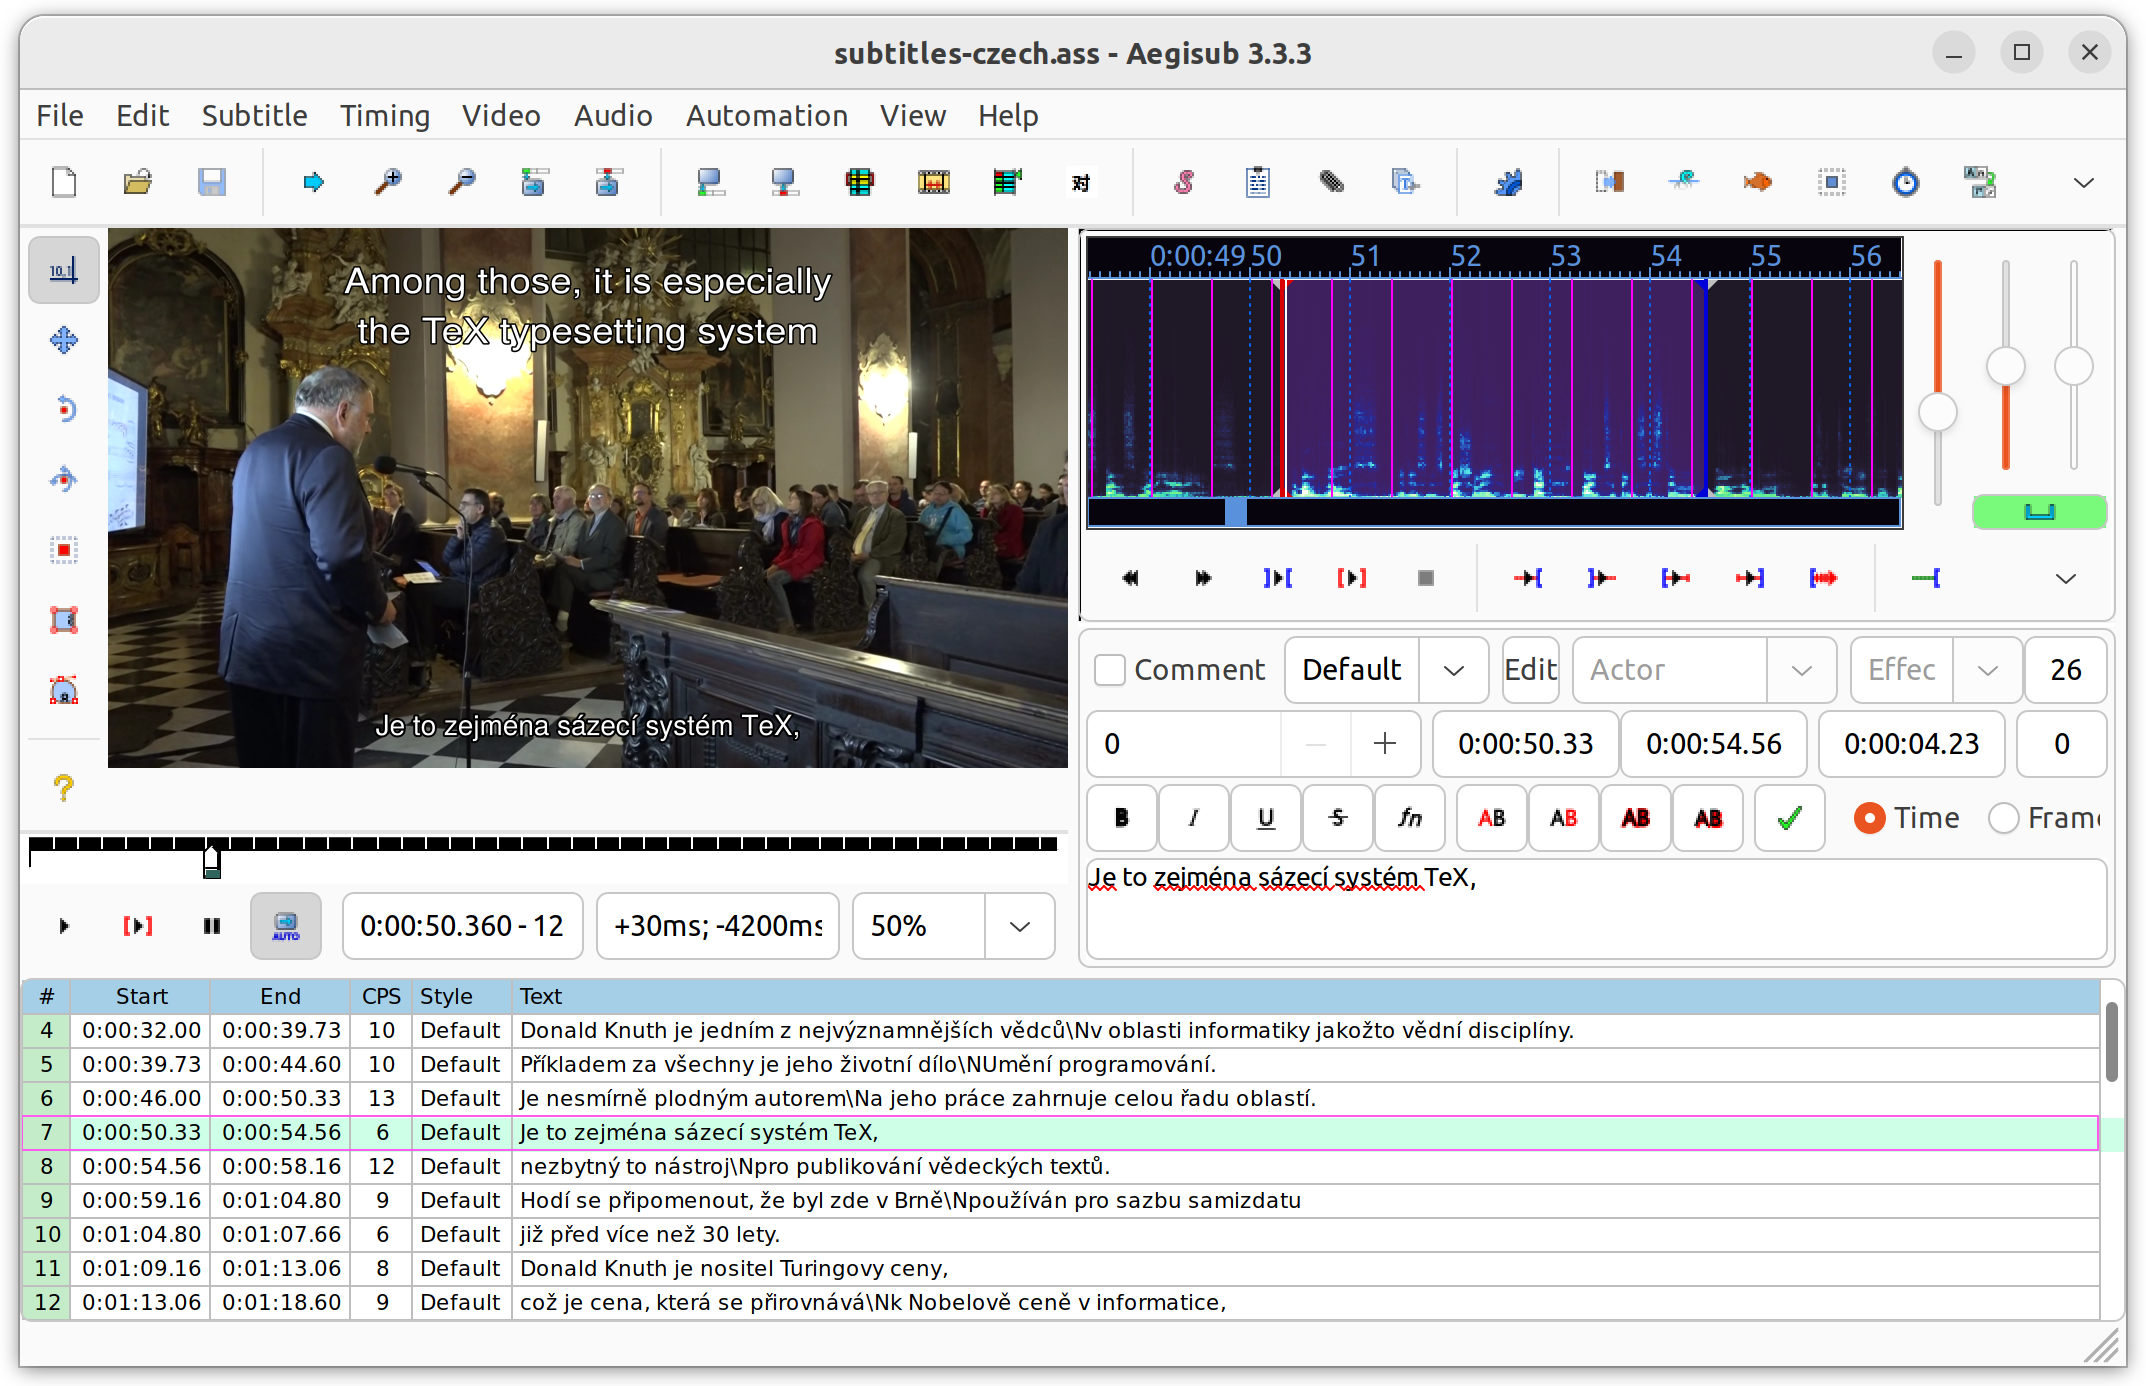
\includegraphics[width=\linewidth]{aegisub}
\caption{Příprava titulků úvodního slova ve svobodném programu Aegisub.}
\end{sideways-figure}

\section{Příprava panelů doprovázejících varhanní oratorium}
\label{sec:panely}

Představení doprovázela projekce na dvou panelech: První panel zobrazoval text Janovy Apokalypsy v novozákonní řečtině a anglickém překladu a druhý panel zobrazoval ilustrace Duane Bibbyho.

Ve videozáznamu jsme panely oproti představení obohatili takto:
\begin{enumerate}
\item Do panelu s textem jsem přidal český překlad Janovy Apokalypsy.
\item Navýšil jsem rozlišení ilustrací od Duane Bibbyho.
\item Změny textu a ilustrací na prvních dvou panelech jsem ozvláštnil animací.
\item Tomáš Szaniszlo připravil třetí panel, který zobrazuje noty pro varhany.
\end{enumerate}

V této sekci popisuji proces přípravy panelů použitých ve videozáznamu.

\input images/screen2-texts

\subsection{Příprava panelu s trojjazyčným textem Zjevení Janova}
Pro řecký a anglický text jsem použil \acro{PDF} dokument~\cite{morland2018fantasia} z kanadské premiéry, který zobrazuje nejprve řecký text na světle žlutém poli a pod ním anglický text na modrém poli, vizte Obrázek~\ref{fig:screen2-texts-greek-and-english-original}.

Aby řecký a anglický text tvořily horní dvě barvy české trikolory, nejprve jsem \acro{PDF} dokument dekomprimoval svobodným nástrojem \acro{PDF}tk~\cite{pdftk}. Následně jsem pomocí \acro{POSIX}ového editoru \texttt{sed} upravil barvu textu a pozadí v dekomprimovaném dokumentu tak, aby byl anglický text na červeném poli, vizte Obrázek~\ref{fig:screen2-texts-greek-and-english-updated}.

Pro český text jsem se svolením České biblické společnosti použil český ekumenický překlad. Pomocí \TeX u, písma Slabo od písmolijny Tiro Typeworks a nástroje ImageMagick~\cite{imagemagick} jsem vytvořil dokument, který vzhledově odpovídá řeckému a anglickému textu a který zobrazuje text na modrém poli, vizte Obrázek~\ref{fig:screen2-texts-czech}.

\subsection{Příprava panelu s ilustracemi Duanea Bibbyho}
Ilustrace Duanea Bibbyho~\cite{bibby2018fantasia} jsem nejprve extrahoval z dokumentu \acro{PDF} pomocí svobodného nástroje pdf\/images. Poté jsem navýšil jejich rozlišení pomocí nástroje waifu2x podobně jako na Obrázku~\ref{fig:waifu2x}:
\begingroup
\small
\begin{verbatim}
$ pdfimages -png fant-screen1-art.pdf ilustrace/ilustrace
$ find ilustrace/ -name '*.png' | sort > ilustrace.txt
$ th waifu2x.lua -l ilustrace.txt -model_dir models/anime_style_art_rgb \
>                -noise_level 3 -tta 1 -o zvětšené-ilustrace/%06d.png
\end{verbatim}
\endgroup

\subsection{Animace panelů s textem a ilustracemi}
Nejprve jsem pro všechny následující páry obrázků z panelů s textem a ilustracemi vygeneroval nástrojem FFmpeg videa s animacemi přechodu, vizte Obrázek~\ref{fig:transition}.

\input images/transition/figure

Posléze jsem obrázky z panelů s textem a ilustracemi synchonizoval se zvukem představení ve svobodném programu Flowblade~\cite{flowblade} pro digitální střih videa, vizte Obrázek~\ref{fig:flowblade}.%
\begin{sideways-figure}{fig:flowblade}
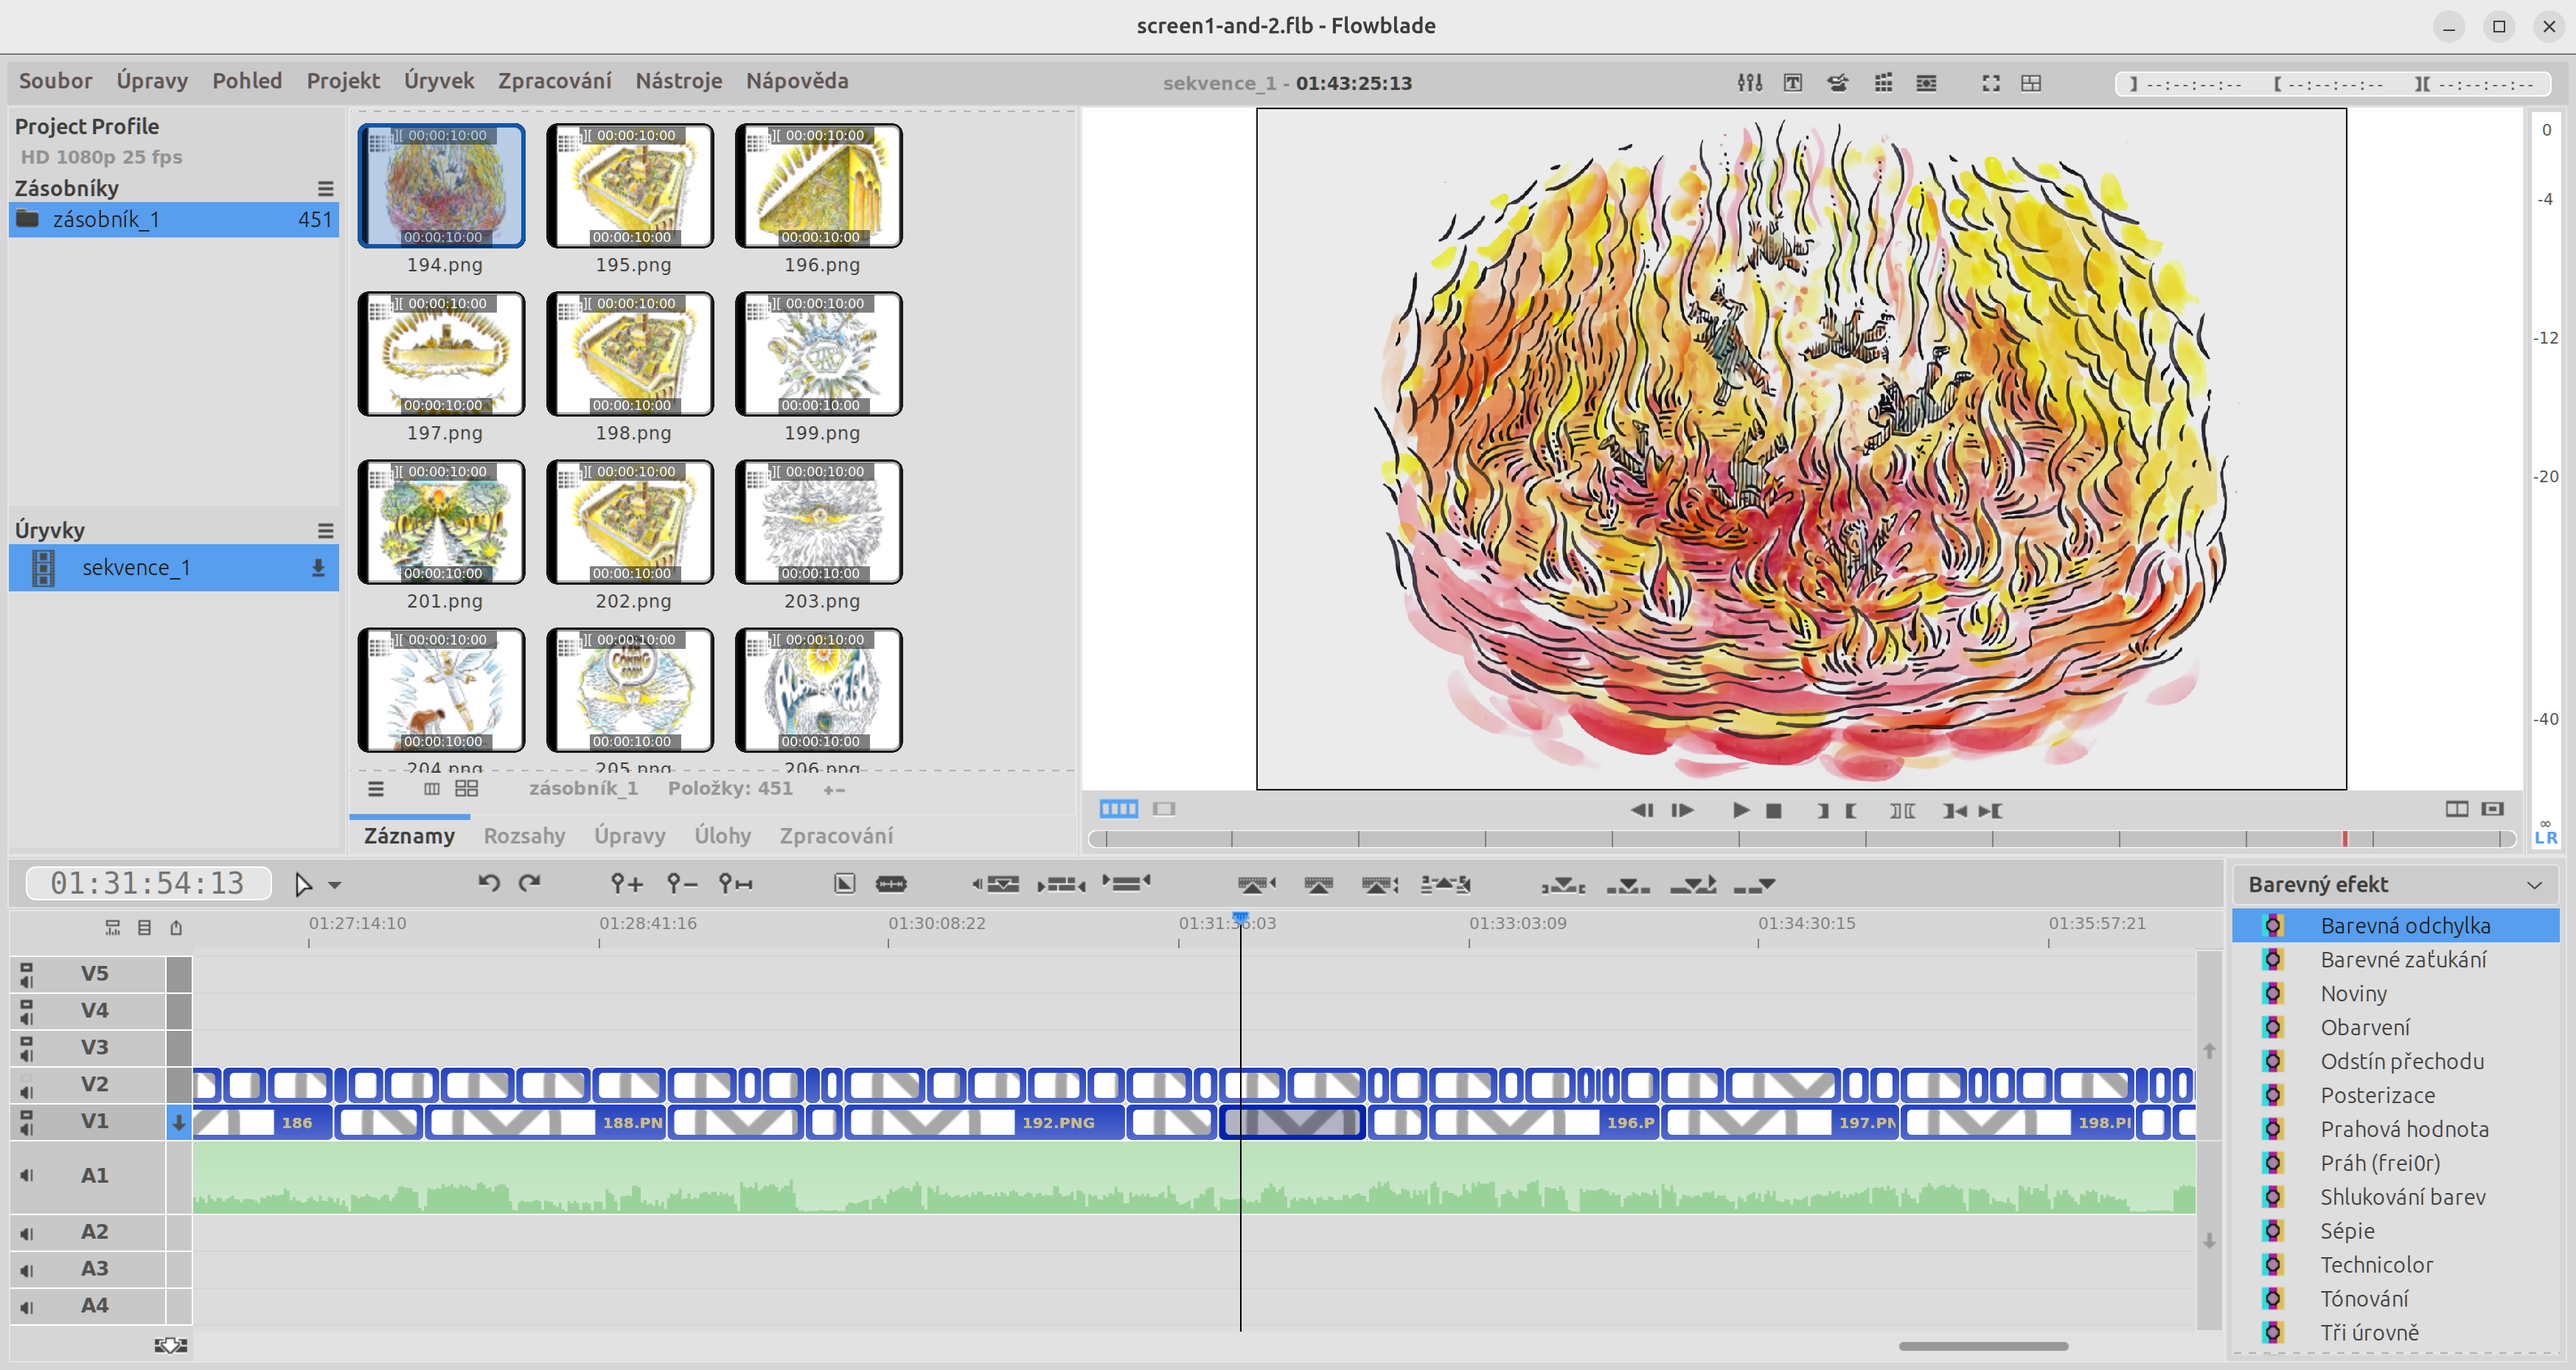
\includegraphics[width=\linewidth]{flowblade}
\caption{Synchronizace panelů s textem a ilustracemi se zvukem představení ve svobodném programu Flowblade.}
\end{sideways-figure}
Projekt Flowblade jsem exportoval do souboru \acro{XML} ve formátu používaném svobodnou softwarovou knihovnou \acro{MLT}~\cite{mlt} pro střih videa. Z tohoto souboru jsem pomocí následujícího programu v jazyce Python~3 extrahoval soubory se seznamem obrázků a dobou jejich trvání vyčíslenou v snímcích videa:

\begin{mintedblock}
\begingroup
\small
\begin{minted}{python}
import xml.etree.ElementTree as ET
from pathlib import Path

obrazky = {}
strom = ET.parse('vstupní-projekt.xml')
for producer in strom.findall('.//producer'):
    obrazek = Path(producer.find('property[@name="resource"]').text)
    producer_id = producer.attrib['id']
    entry = strom.find(f'.//playlist/entry[@producer="{producer_id}"]')
    trvani = int(entry.attrib['out']) - int(entry.attrib['in']) + 1
    obrazky[obrazek] = trvani

with open('časování-ilustrací.txt', 'wt') as f1, \
        open('časování-řeckého-a-anglického-textu.txt', 'wt') as f2, \
        open('časování-českého-textu.txt', 'wt') as f3:
    for obrazek, trvani in sorted(obrazky.items()):
        if obrazek.parent.name == 'ilustrace':
            print(f'{obrazek.name}\t{trvani}', file=f1)
        elif obrazek.parent.name == 'řecký-a-anglický-text':
            print(f'{obrazek.name}\t{trvani}', file=f2)
            print(f'{obrazek.name}\t{trvani}', file=f3)
\end{minted}
\endgroup
\end{mintedblock}

Jeden řádek výstupního souboru \texttt{časování-ilustrací.txt} je např. \texttt{194.png 1119}. To znamená, že obrázek \texttt{ilustrace/194.png} s ilustrací verše 21:8 trvá 1\,119 snímků videa, což je při frekvenci 50 snímků za sekundu přibližně 22 sekund.

Pro každý obrázek jsem vybral animaci podle jeho doby trvání:
\begin{itemize}
\item Po obrázcích kratších než 2 sekundy následuje okamžitě další obrázek.
\item \textls[-15]{Po obrázcích dlouhých 2–5 sekund následuje krátká animace přechodu (520\,ms).}
\item Po obrázcích delších než 5 sekund následuje dlouhá animace přechodu (1\,s).
\end{itemize}
Např. po obrázku \verb|ilustrace/194.png| následuje dlouhá animace přechodu.

Dále jsem pro každý obrázek nástrojem FFmpeg vygeneroval video, jehož délka odpovídala době trvání obrázku po odečtení doby trvání animace. Např. video pro obrázek \verb|ilustrace/194.png| trvá 1\,119 snímků videa po odečtení jedné sekundy pro dlouhou animaci přechodu:
\begin{verbatim}
$ ffmpeg -loop 1 -framerate 50 -i ilustrace/194.png              \
>        -t $(bc -l <<< '1119 / 50 - 1')                         \
>        -r 50 výstupní-video-pro-verš-21-08.mp4
\end{verbatim}

Nakonec jsem videa obrázků a videa animací spojil nástrojem FFmpeg do tří animovaných videí s řeckým a anglickým textem, českým textem a ilustracemi~\cite{ffmpeg-concat}.

\subsection{Příprava panelu s notami pro varhany}
Pro každou z 22 kapitol si Tomáš Szaniszlo na notebooku otevřel digitalizované noty pro varhany~\cite[sekce~„Music scores to download“]{knuth2023fantasia} v prohlížeči \acro{PDF} dokumentů a začal zaznamenávat obrazovku počítače. Následně si Tomáš pustil zvuk představení a pomocí trackpadu posouval noty tak, aby zobrazená část odpovídala zvuku. Výsledkem bylo 22 videí not pro varhany, vizte Obrázek~\ref{fig:screen3}.
\begin{sideways-figure}{fig:screen3}
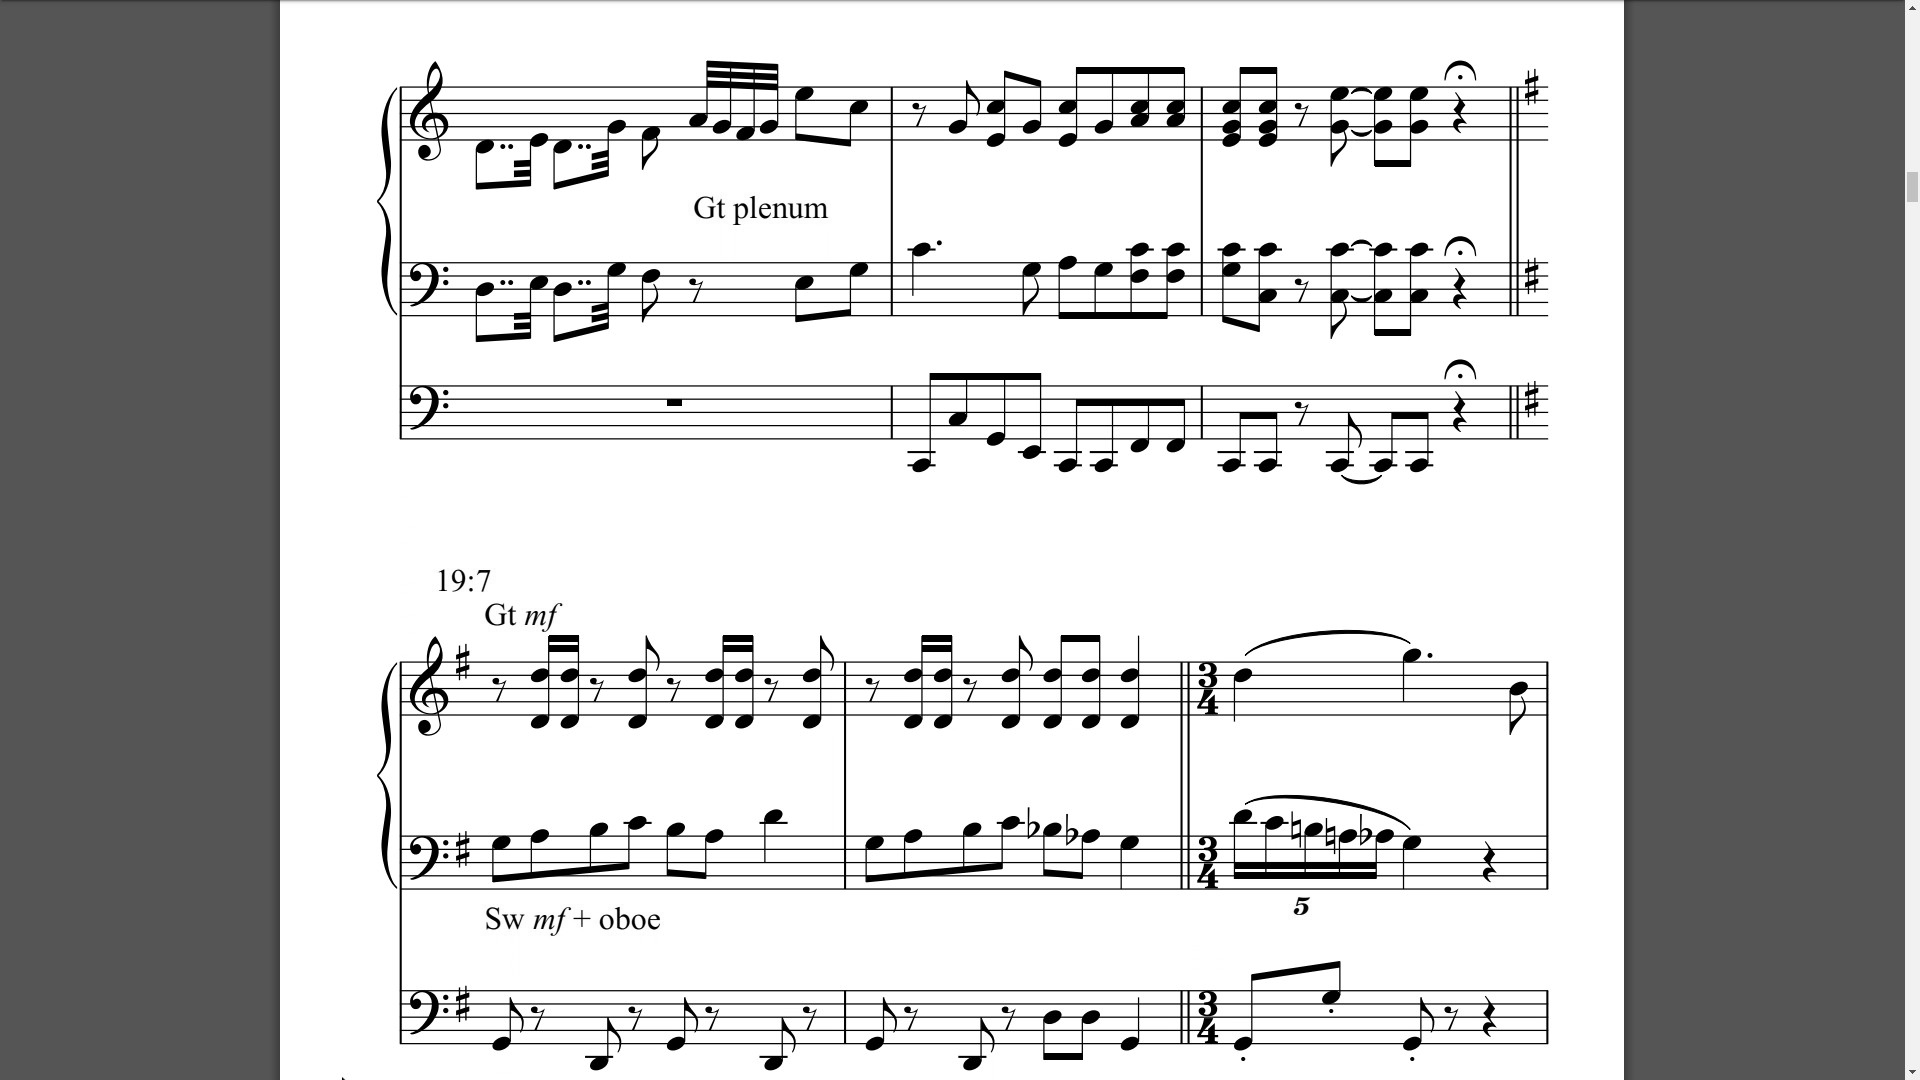
\includegraphics[width=\linewidth]{screen3}
\caption{Videozáznam not pro varhany od Tomáše Szaniszla.}
\end{sideways-figure}

Tato videa jsem nástrojem FFmpeg seřízl z 1920\,px na 1344\,px, aby zmizely postranní šedivé okraje:
\begin{verbatim}
$ ffmpeg -i vstupní-video.mp4                                    \
>        -vf 'crop=1344:1076:280:4,
>             pad=w=1920:h=1076:x=ow-iw/2:y=oh-ih/2:color=white' \
>          výstupní-video.mp4
\end{verbatim}

Dále jsem do horní části videí doplnil bílý obdélník o výšce 62\,px, který na začátku videa překrývá horní šedivý okraj a pak se změní na poloprůhledný obdélník, který přechází od plné neprůhlednosti ve své horní části po plnou průhlednost ve své spodní části a tvoří tak měkký předěl mezi notami a ilustracemi:
\begin{Verbatim}[commandchars=|\{\}]
$ ffmpeg -i vstupní-video.mp4 \
>        -vf "drawbox=0:0:1920:62:white:fill:enable='lte(n,$N|footnotemark{})',
>             drawbox=0:0:1920:1:white@1.0000:enable='gt(n,$N)',
>             drawbox=0:1:1920:1:white@0.9838:enable='gt(n,$N)',
>             drawbox=0:2:1920:1:white@0.9677:enable='gt(n,$N)',
>             ...
>             drawbox=0:61:1920:1:white@0.016:enable='gt(n,$N)'" \
>          výstupní-video.mp4
\end{Verbatim}
\footnotetext{Proměnná \texttt{\$N} značí snímek, po kterém se obdélník změní na poloprůhledný, a liší se pro jednotlivá videa not. Např. ve videu pro 21. kapitolu jsem nastavil \texttt{N=2700}. Při frekvenci 50 snímků za sekundu tedy dojde ke změně po 54 sekundách, kdy již Tomáš posunul noty tak, že horní šedivý okraj není vidět.}

Poté jsem videa sestříhal a synchonizoval se zvukem představení v programu Flowblade podobně jako v předchozí sekci. Výsledné video jsem vykreslil nástrojem Melt z knihovny \acro{MLT}:
\begin{verbatim}
$ melt vstupní-projekt.xml -consumer avformat:výstupní-video.mp4 \
>      vcodec=libx265 crf=17 preset=veryslow pix_fmt=yuv420p     \
>      acodec=aac ab=384k ar=44100
\end{verbatim}

Pro srovnání surových videí not s výsledným videem vizte obrázky~\ref{fig:screen3} a \ref{fig:montage}.

\section{Spojení jednotlivých částí do výsledného videa}
\label{sec:spojeni}
Nejprve jsem videa panelů s textem, ilustracemi a notami pro varhany spojil podle diagramu na Obrázku~\ref{fig:montage-diagram}:
\begin{sideways-figure}{fig:montage-diagram}
\centering
\input images/montage-diagram
\caption{Diagram pro spojení jednotlivých panelů do výsledného videa.}
\ClassWarning{csbulletin}{Make sure that the captions on the left and right sides of the diagram are facing down in the final article}
\end{sideways-figure}
\begin{sideways-figure}{fig:montage}
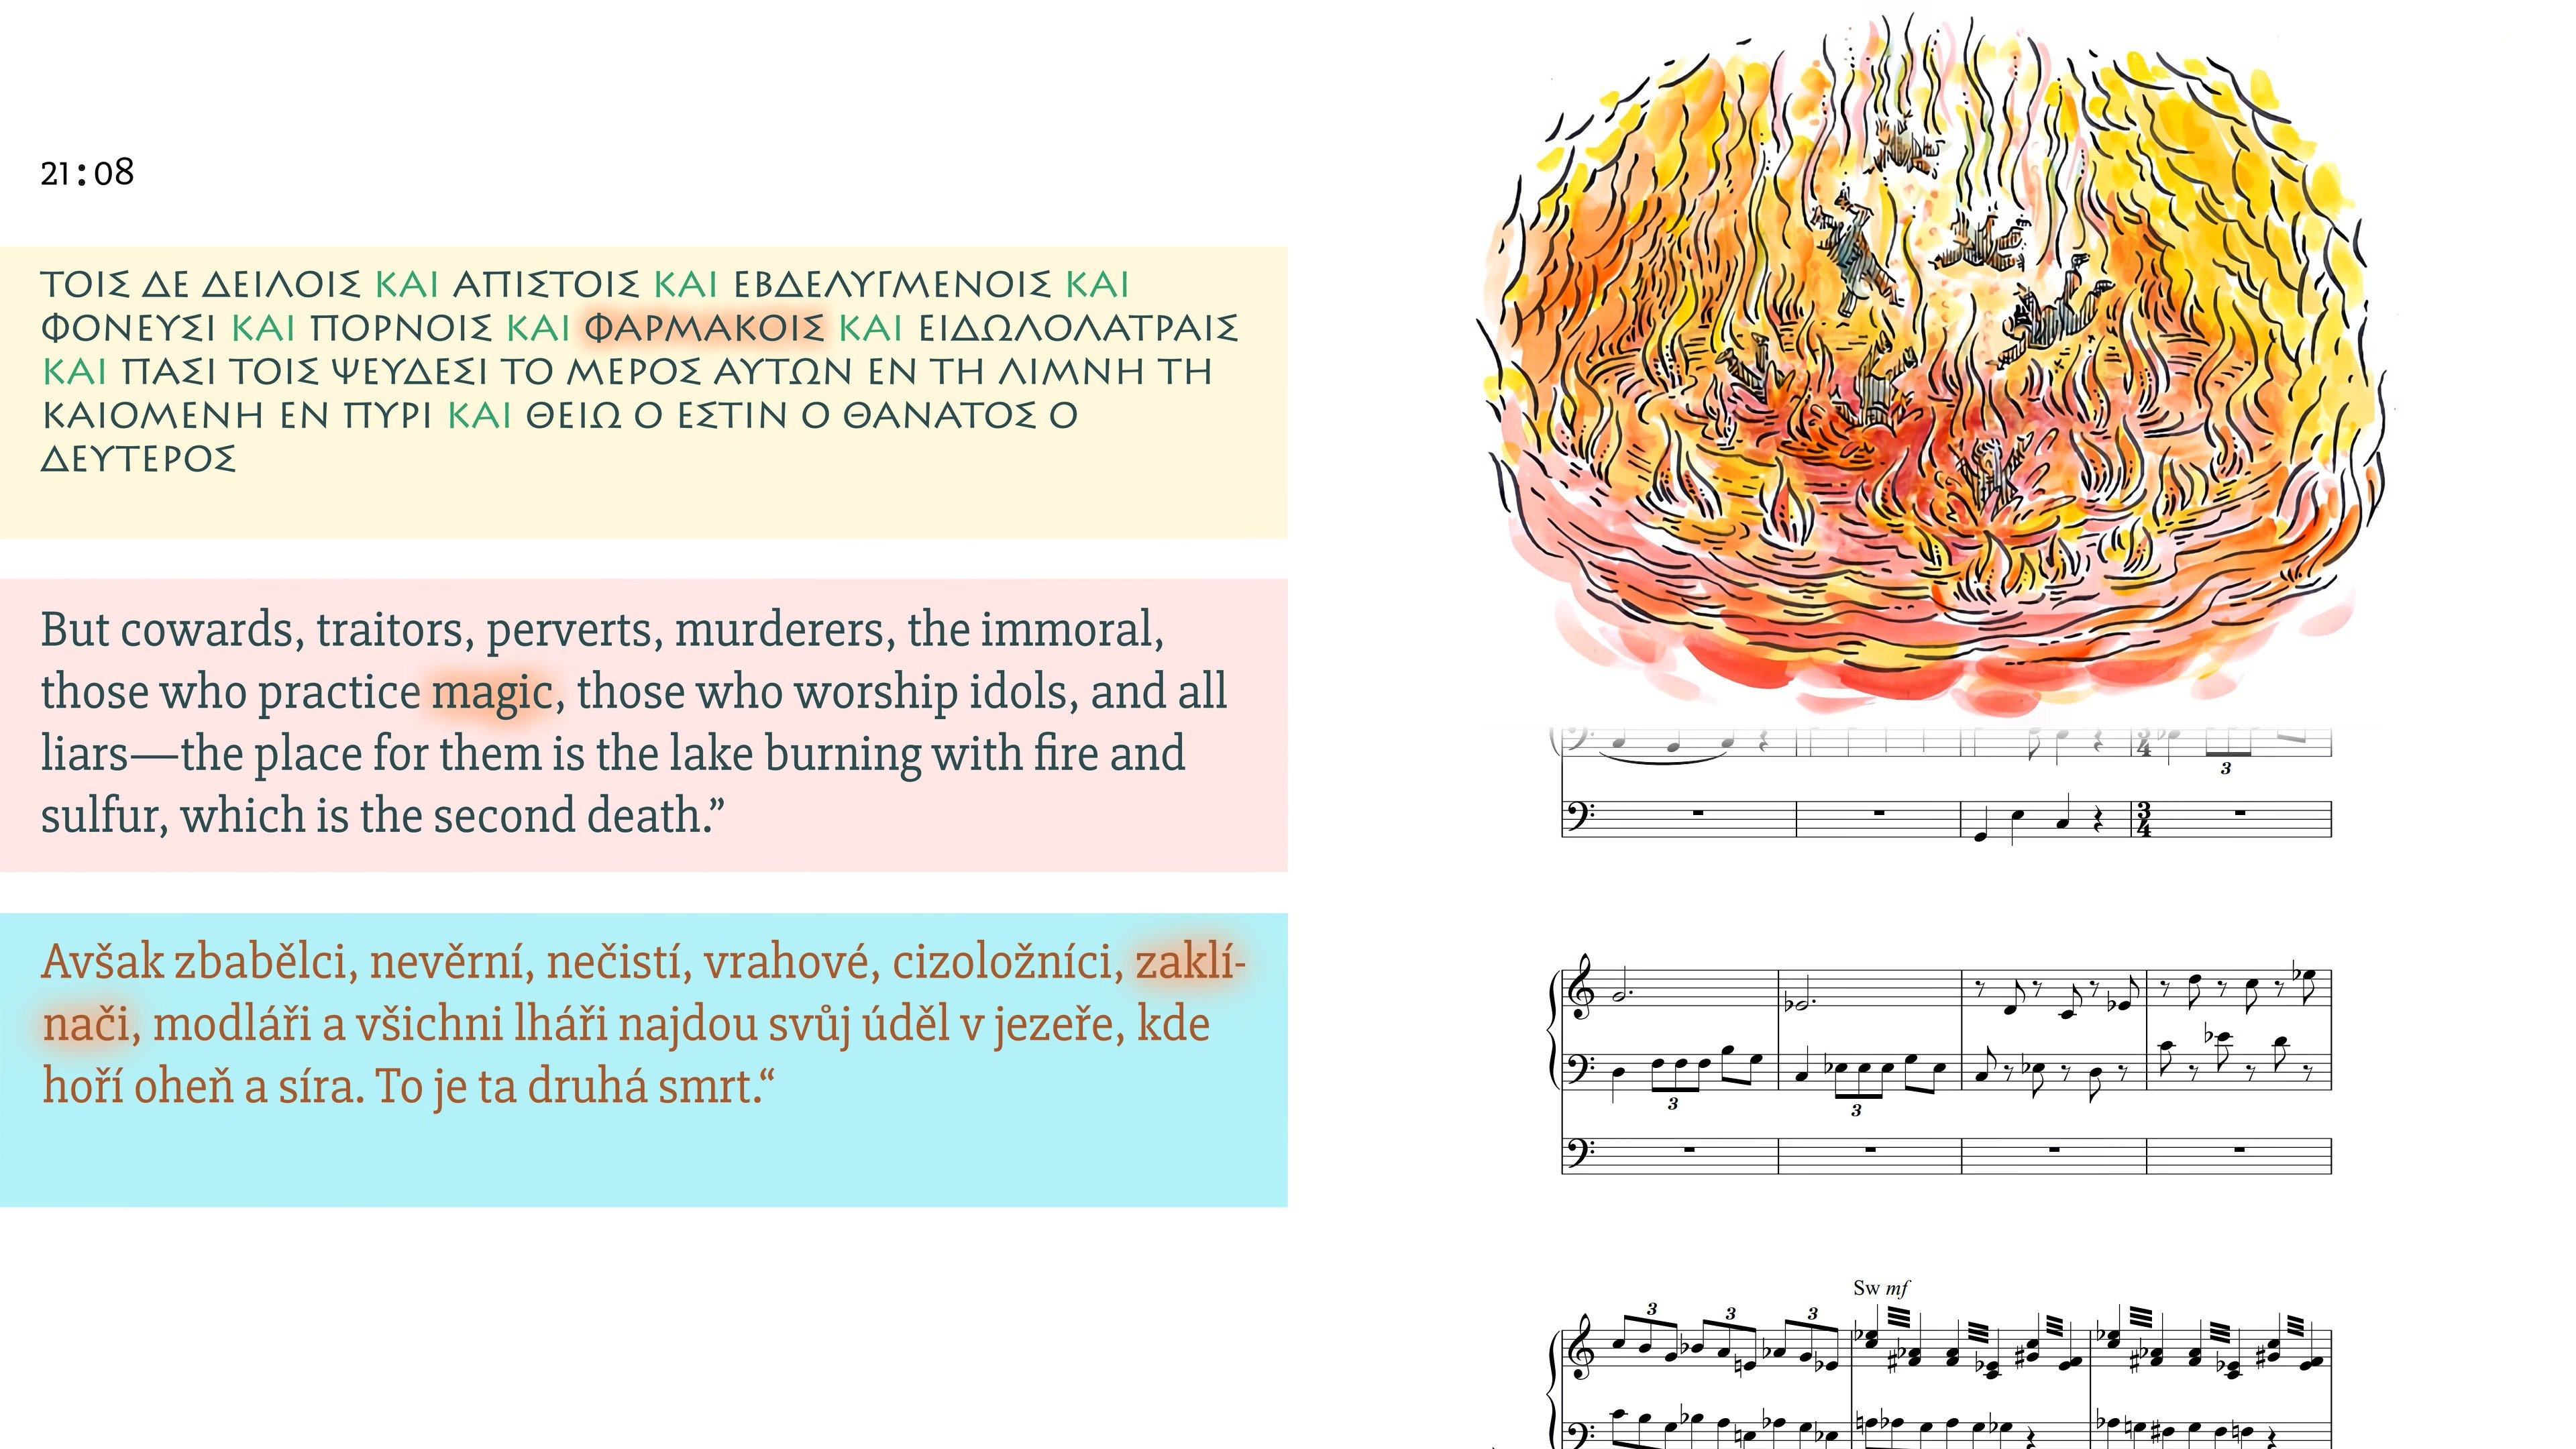
\includegraphics[width=\linewidth]{montage}
\par\vspace{-1.175cm}
\caption{Výsledné video.\kern 8.5cm\relax}
\end{sideways-figure}
\begin{verbatim}
$ ffmpeg -f lavfi -i color=c=white:s=3840x2160:rate=50 \
>        -i vstupní-video-s-řeckým-a-anglickým-textem.mp4 \
>        -i vstupní-video-s-českým-textem.mp4 \
>        -i vstupní-video-s-ilustracemi.mp4 \
>        -i vstupní-video-s-notami-pro-varhany.mp4 \
>        -filter_complex '
>            [0:v]null[pozadi]; [1:v]null[recky-a-anglicky-text];
>            [2:v]crop=1920:960:0:63[cesky-text];
>            [3:v]pad=1920:1084:ow-iw/2:oh-ih/2:white[ilustrace];
>            [4:v]crop=1344:1076:280:4,
>                 pad=1920:1076:ow-iw/2:oh-ih/2:white[noty];
>            [pozadi][recky-a-anglicky-text]overlay=0:160[kolaz1];
>            [kolaz1][cesky-text]overlay=0:1360[kolaz2];
>            [kolaz2][noty]overlay=1920:1084[kolaz3];
>            [kolaz3][ilustrace]overlay=1920:0[kolaz]' \
>        -map '[kolaz]' -t 01:43:25 -r 50 výstupní-video.mp4
\end{verbatim}
Potom jsem k výsledku připojil videozáznam úvodního slova a závěru~\cite{ffmpeg-concat}. Obrázek~\ref{fig:montage} ukazuje výsledné video.

\section{Závěr}
\label{sec:zaver}
18. prosince 2019 se v posluchárně \acro{D3} na \acro{FI~MU} konalo promítání videozáznamu představení, vizte Obrázek~\ref{fig:screening}.%
\begin{sideways-figure}{fig:screening}
\centering
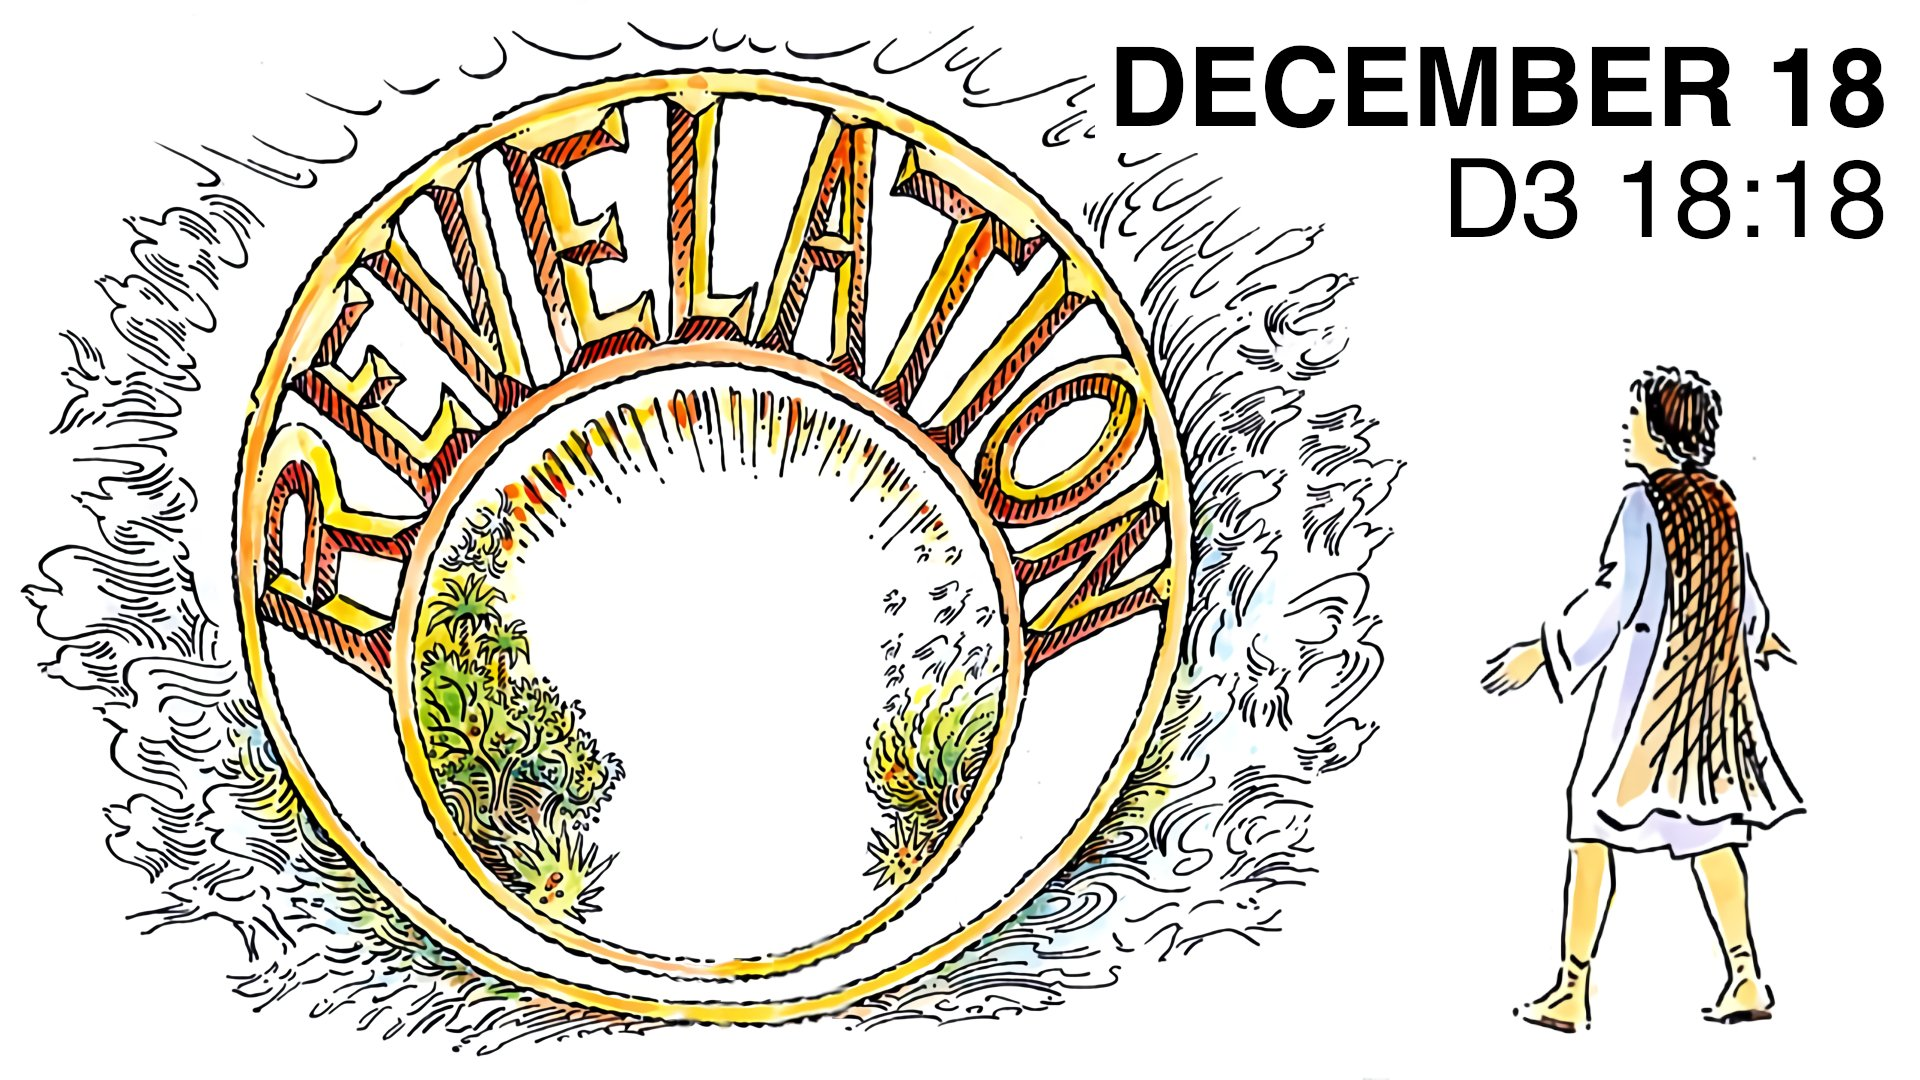
\includegraphics[width=\linewidth]{images/2019-12-18_revelation}
\caption{Plakát zvoucí studující a zaměstnance \protect\acro{FI~MU} na promítání videozáznamu přestavení.}
\end{sideways-figure}

Před začátkem promítání spustil Tomáš Szaniszlo přes piezoelektrické reproduktory integrované na základních deskách počítačů v počítačové hale digitalizovanou verzi hudby, která při představení doprovází verš 2:1 Zjevení. Zároveň zobrazil na monitorech všech počítačů v hale zprávu: „Přijďte na promítání v \acro{D3} o 18:18“~\cite{knuth-fantasia-verse-2-1}. Překvapené studující následně dovedl do posluchárny autor článku, přestrojený za proroka Jana.

Videozáznam byl zveřejněn na YouTube kanálu \acro{FI~MU} 1. ledna 2020~\cite{fimu2020czech}.

\begingroup
\sloppy
\printbibliography
\endgroup

\begin{summary}
On October 11, 2019, the Czech premiere of the ``Fantasia Apocalyptica'' multimedia work was held for the 25th anniversary of Masaryk University's Faculty of Informatics, featuring its author, Donald Knuth. A video recording of the perfomance was taken and published at the YouTube channel of the Faculty of Informatics.
\oldlooseness=-1

In this article, I describe how the recording was prepared from processing the raw footage through replicating the panels that accompanied the performance to the final composition. Apart from super-resolution imaging, the editing of the intro and the wrap-up, and the compression of sound, only free open-source tools like \TeX, Audacity, Aegisub, FFmpeg, \acro{MLT}, \acro{PDF}tk, and ImageMagick were used. In the article, I describe how readers can use these tools for their own recordings.

\keywords: footage acquisition, audio-visual production, subtitles, \TeX, \\ Audacity, Aegisub, \acro{ASS}, FFmpeg, ImageMagick, \acro{MLT}, \acro{PDF}tk, waifu2x
\end{summary}

\end{document}